\begin{frame}[allowframebreaks]{Transfer Learning}
\begin{itemize}
    \item \textbf{What is Fine-Tuning?}  
    \begin{itemize}
        \item A strategy in \textbf{transfer learning} where a pre-trained model is adapted to a new task.
        \item Instead of training from scratch, we start from a model already trained on a related task.
    \end{itemize}
    \item \textbf{Why use Fine-Tuning?}  
    \begin{itemize}
        \item Saves time and computational resources.
        \item Improves performance, especially with limited data.
    \end{itemize}
\end{itemize}
\end{frame}

\begin{frame}[allowframebreaks]{When to fine-tune your model?}
    \begin{itemize}
        \item New dataset is small + similar distribution to original dataset:
        \begin{itemize}
            \item Freeze (or partially freeze) feature extraction layers and fine-tune the classifier.
        \end{itemize}
        \item New dataset is small + different distribution to original dataset:
        \begin{itemize}
            \item Use the pretrained network as a generic feature extractor and train a light classifier on top (e.g., SVM).
            \item In modern practice, you might also freeze earlier layers and selectively fine-tune later layers.
        \end{itemize}
        \item New dataset is large, regardless of the original data distribution:
        \begin{itemize}
            \item Fine-tune the entire network (both features extractor and classifier).
        \end{itemize}
    \end{itemize}
\end{frame}

\begin{frame}{Finetuning}
    \begin{figure}
    \centering
    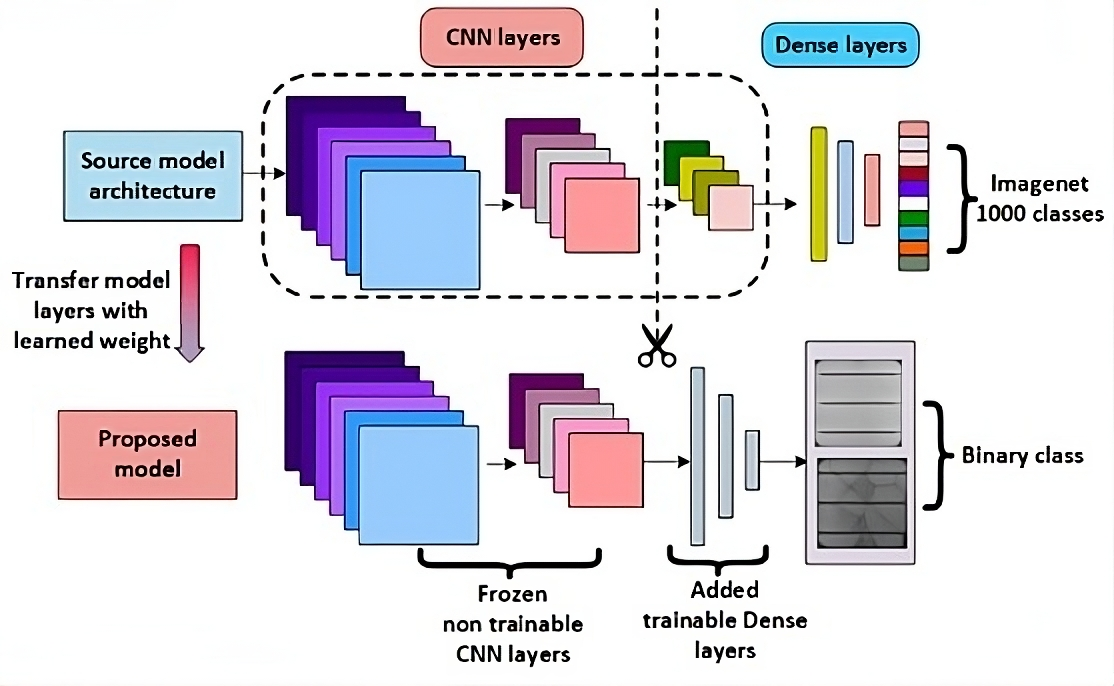
\includegraphics[width=1.0\textwidth,height=1.0\textheight,keepaspectratio]{images/Finetuning_fig.png}
    \caption{Learning and Transferring Mid-Level Image Representations using Convolutional Neural Networks }
    \end{figure}
\end{frame} 